\documentclass{article}
% \usepackage{covergraphic}
\usepackage{graphicx}
\usepackage{ragged2e}
\usepackage{xcolor}
\colorlet{coverdarkcolor}{black}
\definecolor{coverbgcolor}{RGB}{212,175,55}  % gold
\definecolor{coverboldcolor}{RGB}{0,67,37}  % green
% \definecolor{coverboldcolor}{RGB}{103,0,153}  % purple

\usepackage[defaultsans]{lato}

\usepackage{stackengine}
\renewcommand{\stackalignment}{c}

% I want the booleans offered by this package
\usepackage{etoolbox}
% Guidelines help to arrange the parts visually.  Show or not?
\newbool{showguidelinesbool}
  % set the default by uncommenting one or the other
  % \booltrue{showguidelinesbool} 
  \boolfalse{showguidelinesbool}  
% You can cause guidelines to be shown by invoking with
%   pdflatex "\def\showguidelines{}\setlength{\unitlength}{1in}
\begin{picture}(0,0)(1.25,-1.15)
  \put(0,-11){\makebox[0in][l]{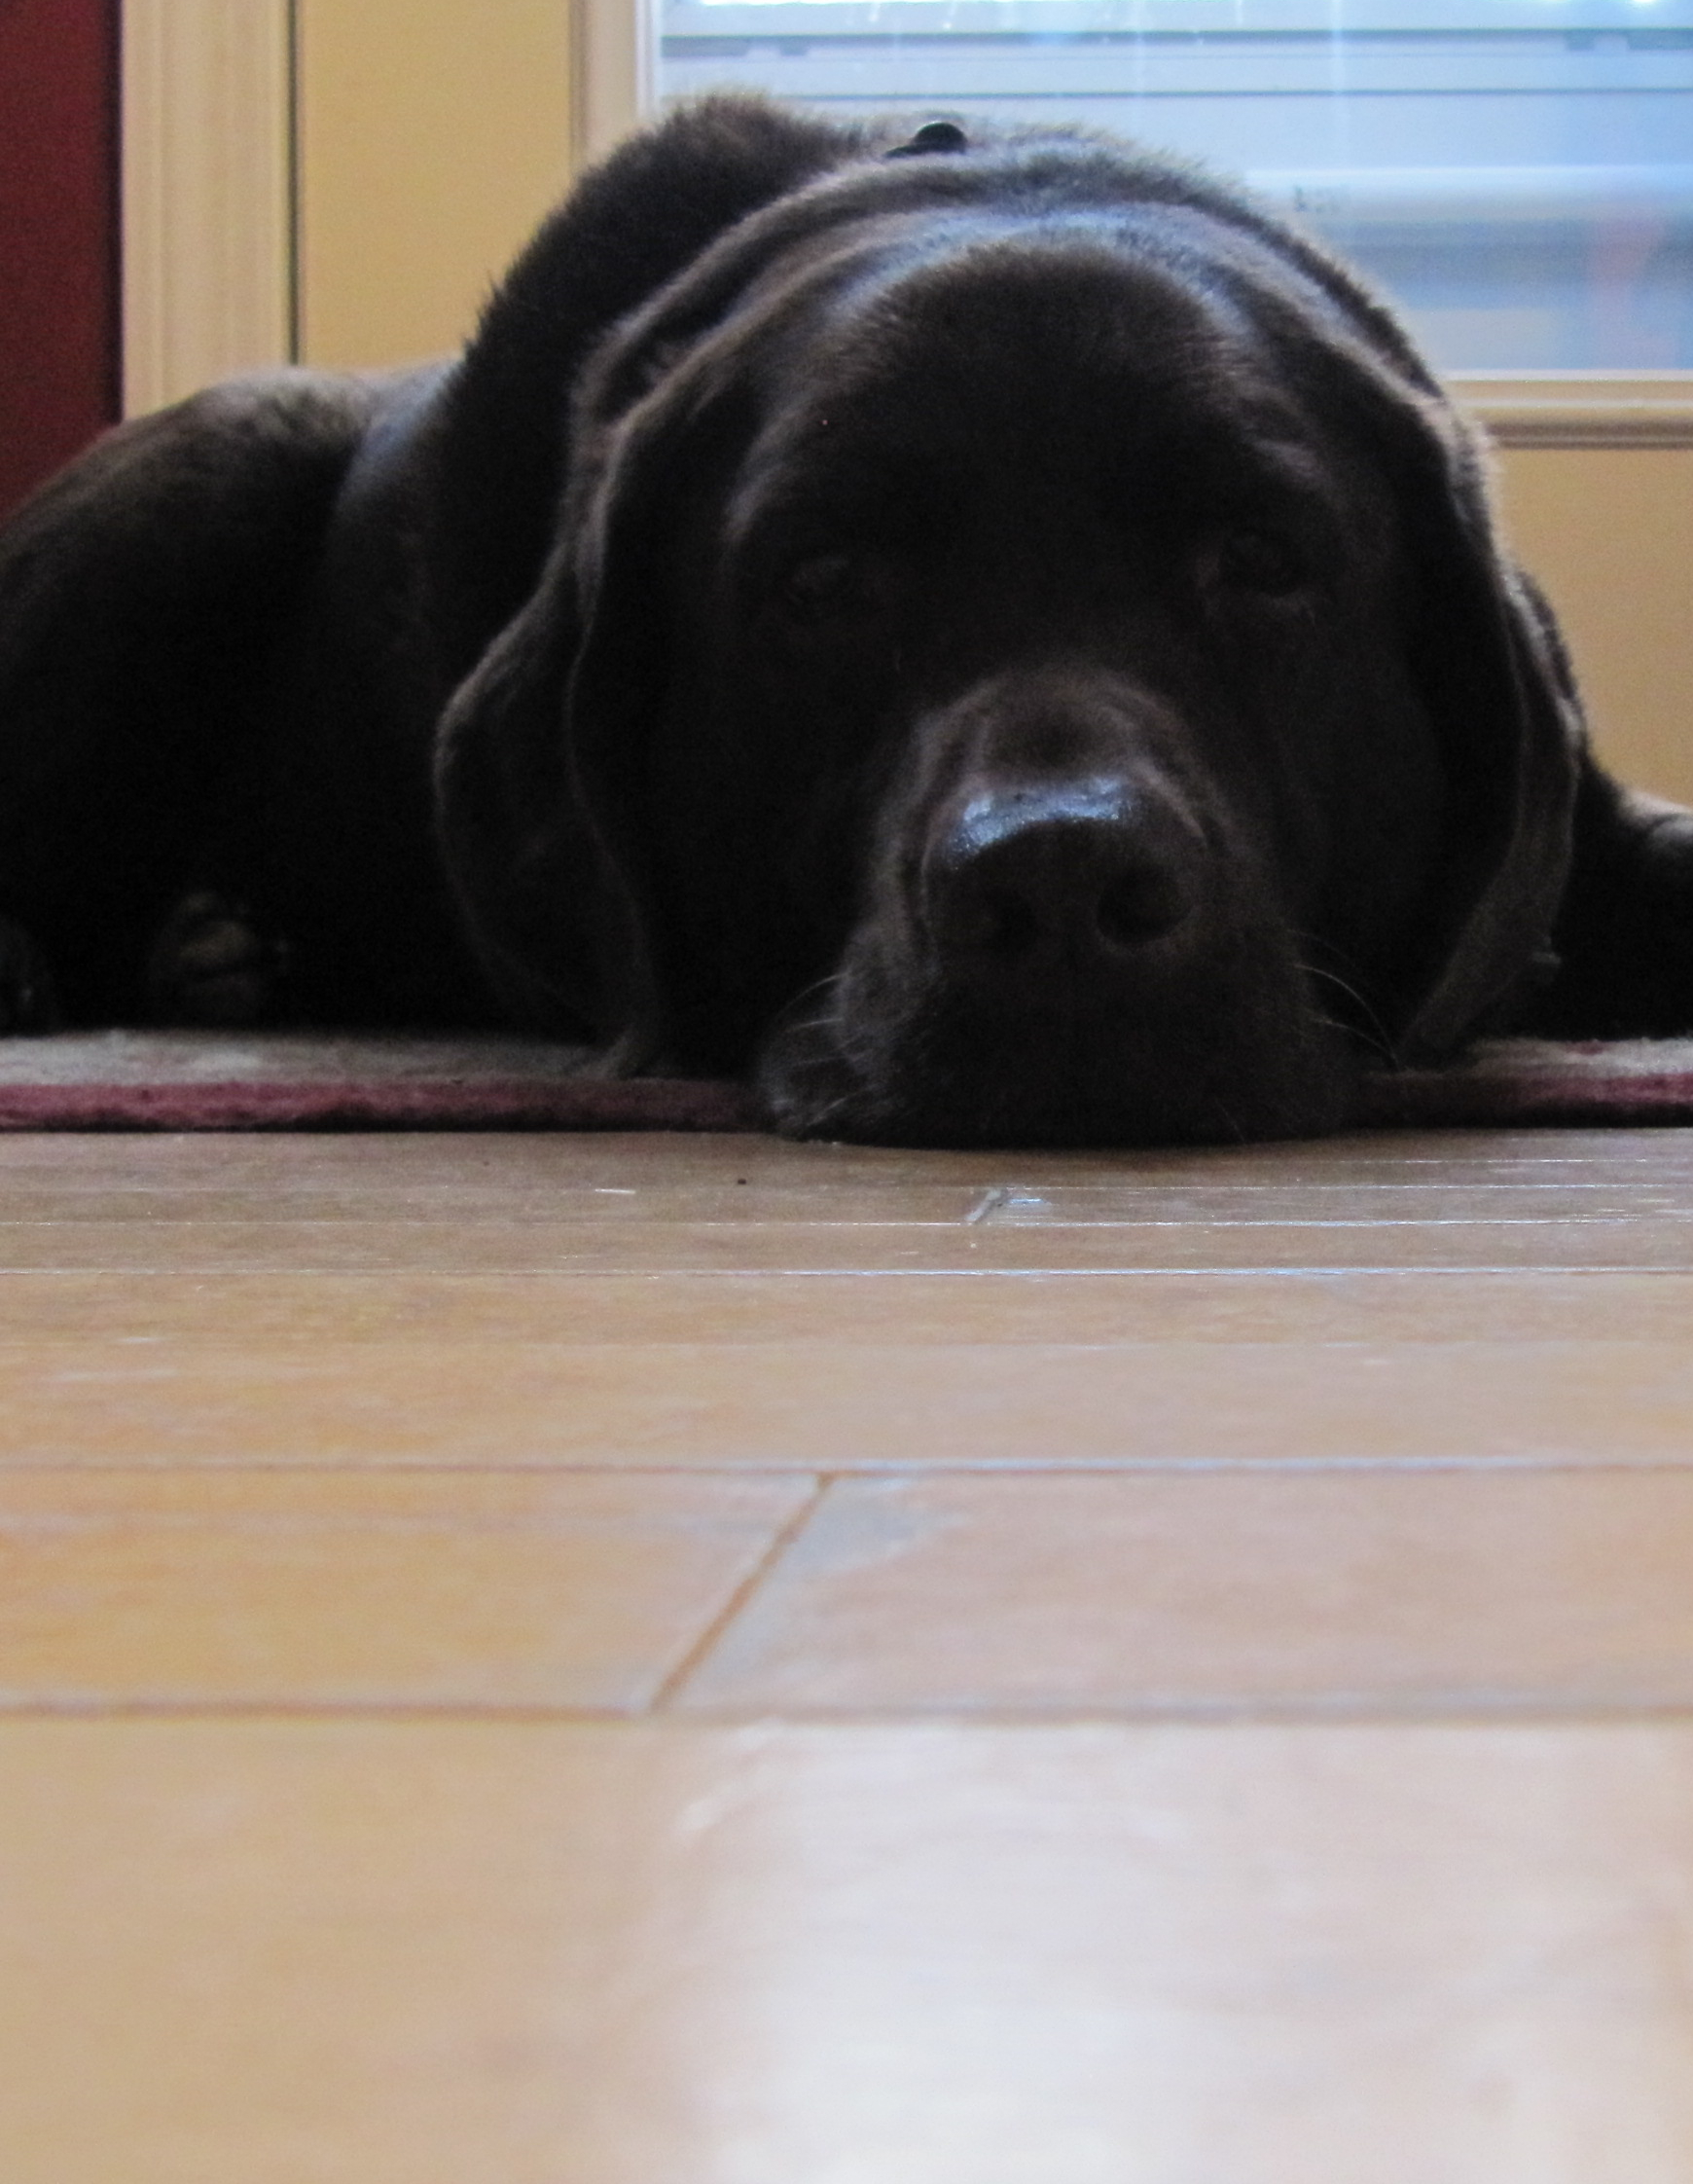
\includegraphics[height=11in]{pix/suzy_cover.jpg}}}
  \put(4.25,-9.45){\sffamily \begin{tabular}{l} 
                            \Huge\bf Lab Manual  \\[.2ex]
                            \large \hspace*{0.3em}for \\[.3ex]
                            \LARGE Linear Algebra \\[.2ex]
                            \large \hspace*{0.3em}by \\[.4ex]
                            \Large Jim Hef{}feron
                          \end{tabular}}
\end{picture}
\newpage
\thispagestyle{empty}
\vspace*{\fill}
\begin{center}
\textit{Cover:} our Chocolate Lab, Suzy.
\end{center}
\endinput
"
% See http://stackoverflow.com/a/1466610
\ifdefined\showguidelines
  \booltrue{showguidelinesbool}
\fi
\ifbool{showguidelinesbool}{\typeout{!!! GUIDELINES SHOWN}}{}

% Size of page
\newlength{\totalcoverwidth} \setlength{\totalcoverwidth}{15.0in} % 7.5+7.5
\newlength{\spinewidth} \setlength{\spinewidth}{1in}
\addtolength{\totalcoverwidth}{\spinewidth}
\usepackage[papersize={16in,9.25in},margin=0in]{geometry}  

% \newcommand{\spinetext}[1]{\color{black}\fontsize{40pt}{8pt}{\fontfamily{ugq}\selectfont #1}}
\newcommand{\spinetext}[1]{\color{black}\fontsize{38pt}{8pt}{\fontfamily{ugq}\selectfont #1}}
% \newcommand{\spineauthortext}[2]{\color{coverdarkcolor}\fontsize{#2pt}{8pt}{\fontfamily{ugq}\selectfont{#1}}}
\newcommand{\spineauthortext}[1]{\color{coverdarkcolor}\fontsize{23pt}{8pt}{\fontfamily{ugq}\selectfont{#1}}}
\newcommand{\spine}{%
\setlength{\unitlength}{1in}
\begin{picture}(1,9.5)
  \setstackgap{S}{2.1ex}
  % \put(0.235,5.65){\Shortstack{{\spinetext{L}} {\spinetext{I}} {\spinetext{N}} {\spinetext{E}} {\spinetext{A}} {\spinetext{R}}}}
  \put(0.18,8.5){\rotatebox[origin=lc]{-90}{\spinetext{Linear Algebra}\hspace{01.75in}\spineauthortext{Hefferon}}}
  % \put(0.35,2.5){\rotatebox[origin=lc]{-90}{\spineauthortext{Hefferon}}}
  \setstackgap{S}{0.9ex}
  % \put(0.3925,1.15){\Shortstack{{\spineauthortext{H}{14}} {\spineauthortext{E}{14}} {\spineauthortext{F}{14}} {\spineauthortext{F}{14}} {\spineauthortext{E}{14}} {\spineauthortext{R}{14}} {\spineauthortext{O}{14}} {\spineauthortext{N}{14}}}} % tried fake small caps by making the H be 14 pt, others be 11
\end{picture}
}

\newcommand{\backcovertext}{%
\RaggedRight
\color{black}\fontsize{14pt}{17pt}\fontfamily{fos}\selectfont
\begin{minipage}{5.5in}
%\setlength{\parindent}{2em}
\setlength{\parskip}{1.4ex}
This text covers a standard first course:
Gauss's Method, vector spaces, linear maps and matrices, determinants,
and eigenvalues and eigenvectors.
In addition, each chapter ends with some
brief topics, such as applications.

What sets it apart is careful motivation, 
many examples, and extensive exercise sets.
Together these help each student master the material of
the course, and also help an instructor develop that student's  
level of mathematical maturity.

This book
has been freely available online for many years and is widely used, 
both in classrooms and for self-study.
It is supported by worked answers for all exercises, 
projection slides for classroom use, 
and a lab manual of computer work based on \textit{Sage}. 
\end{minipage}
}

\newcommand{\backcoverhead}{%
\setlength{\unitlength}{1in}
\begin{picture}(0,0)
  \put(1,-.1){{\color{coverbgcolor}\rule{4.4in}{2pt}}}
  \put(0,0){\color{coverboldcolor}\fontsize{25pt}{8pt}\fontfamily{fos}\selectfont \textit{A developmental approach to}}
  \put(2.9,-.45){\color{black}\fontsize{25pt}{8pt}\fontfamily{fos}\selectfont \textbf{Linear Algebra}}
\end{picture}
}

\setlength{\parindent}{0in}
\begin{document}\pagestyle{empty}\thispagestyle{empty}

\newcommand{\frontcovertext}[1]{\color{black}\fontsize{55pt}{8pt}{\fontfamily{ugq}\selectfont #1}}
% \newcommand{\frontcovereditiontext}[1]{\color{black}\fontsize{20pt}{8pt}{\fontfamily{ugq}\selectfont #1}}
\newcommand{\frontcovereditiontext}[1]{\color[gray]{0.4}\fontsize{20pt}{6pt}\fontfamily{ugq}\selectfont \textsf{#1}}
% \newcommand{\frontcovereditiontext}[1]{\color{black}\fontsize{20pt}{6pt}\fontfamily{ugq}\selectfont #1}
\newcommand{\frontcoverauthortext}[1]{\color{black}\fontsize{27.5pt}{6pt}{\fontfamily{ugq}\selectfont #1}}
\newcommand{\frontcoverurltext}[1]{\color[gray]{0.4}\fontsize{18pt}{6pt}\fontfamily{ugq}\selectfont \textsf{#1}}
% \newcommand{\frontcoverurltext}[1]{\color[gray]{0.4}{\lato \fontsize{18pt}{6pt}\fontseries{sb}\selectfont #1}}

\setlength{\unitlength}{1in}
\begin{picture}(0,0) 
  \ifbool{showguidelinesbool}{% 
    \put(0,-1){\makebox[0in]{\color{red}0}}
    \put(1,-1){\makebox[0in]{\color{red}1}}
    \put(2,-1){\makebox[0in]{\color{red}2}}
    \put(3,-1){\makebox[0in]{\color{red}3}}
    \put(4,-1){\makebox[0in]{\color{red}4}}
    \put(5,-1){\makebox[0in]{\color{red}5}}
    \put(6,-1){\makebox[0in]{\color{red}6}}
    \put(7,-1){\makebox[0in]{\color{red}7}}
    \put(7.5,-1){\color{red}\line(0,-1){8}}
    \put(8,-1){\makebox[0in]{\color{red}8}}
    \put(8,-1){\color{blue}\line(0,-1){8}}
    \put(8.5,-1){\color{red}\line(0,-1){8}}
    \put(9,-1){\makebox[0in]{\color{red}9}}
    \put(9.5,-1){\color{blue}\line(0,-1){8}}
    \put(10,-1){\makebox[0in]{\color{red}10}}
    \put(11,-1){\makebox[0in]{\color{red}11}}
    \put(12,-1){\makebox[0in]{\color{red}12}}
    \put(13,-1){\makebox[0in]{\color{red}13}}
    \put(14,-1){\makebox[0in]{\color{red}14}}
    \put(15,-1){\makebox[0in]{\color{red}15}}
    \put(15,-1){\color{blue}\line(0,-1){8}}
    \put(16,-1){\makebox[0in]{\color{red}16}}
  }{} 
  \put(9.1,-7.57){\includegraphics{asy/try.pdf}}
  \put(9.1,-8.5){\includegraphics{asy/shadow.pdf}}
  \put(15,-3){\makebox[0pt][r]{\frontcovertext{Linear Algebra}}}
  \put(15,-3.7){\makebox[0pt][r]{\frontcoverauthortext{Jim Hef{}feron}}}
  \put(15,-7.95){\makebox[0pt][r]{\frontcoverurltext{joshua.smcvt.edu/linearalgebra}}}
  \put(15,-2.20){\makebox[0pt][r]{\frontcovereditiontext{Fourth edition}}}
  % \put(15,-4.25){\makebox[0pt][r]{\frontcovereditiontext{Edition four}}}
  \put(7.5,-9.5){\spine}
  \put(1,-1.1){\backcoverhead}
  \put(1,-3.75){\backcovertext}
\end{picture}
\end{document}
